\documentclass[a4paper,14pt]{extarticle} %the default article class is limited to 12pt, but you can go up to 14, 17 or 20 points if you use the extarticle class:
\usepackage{cmap} %make LaTeX PDF output copy-and-pasteable
\usepackage[T2A]{fontenc}
\usepackage[utf8]{inputenc}
\usepackage[english,ukrainian]{babel}

\usepackage{amssymb,amsfonts,amsmath,cite,enumerate,float}
\usepackage{indentfirst} %set an additional space before a paragraph at the begining of new section
\usepackage{setspace}
\usepackage{textcomp}

\usepackage{geometry} 
\geometry{left=1.25cm}
\geometry{right=1.25cm}
\geometry{top=1cm}
\geometry{bottom=2cm}

\usepackage{graphicx}
\usepackage{wrapfig}
\graphicspath{{images/}} %path to images

\parskip=1mm %space between paragraphs

\usepackage[dvipsnames]{xcolor}
\usepackage{color}
% 1) tutorial about xcolor:  https://www.overleaf.com/learn/latex/Using_colours_in_LaTeX
% 2) huge tutorial about xcolor: https://latex-tutorial.com/color-latex/ 
% 3) RGB calculator: https://www.w3schools.com/colors/colors_rgb.asp

\usepackage{listings} %for code

\lstset{
    frame=single, %lines
    language=Python,
    aboveskip=3mm,
    belowskip=3mm,
    columns=flexible,
    basicstyle={\small\ttfamily},
    numbers=left,
    numberstyle=\tiny\color{gray},
    commentstyle=\color{OliveGreen},
    stringstyle=\color{Mahogany},
    morestring=[b]''',
    showstringspaces=false,
    keywordstyle=\bfseries\color{Blue},
    emph={[1]import, as, for, return}, emphstyle={[1]\color{DarkOrchid}},
    emph={[2]range, abs, built_in, Bresenham, switcher, Up, Down, X, Y}, emphstyle={[2]\color{Sepia}},
    breaklines=true,
    breakatwhitespace=true,
    tabsize=4
}

\begin{document}

\begin{titlepage}
    \newpage

    \begin{minipage}[c]{\linewidth}

        \newlength{\maxpreambula}
        \settowidth{\maxpreambula}{\small{<<Київський політехнічний інститут імені Ігоря Сікорського>>}}    

        \hspace{5cm}\parbox{\maxpreambula}{
            \begin{spacing}{1.1}\small{
                Міністерство освіти і науки України \\
                Національний технічний університет України \\
                <<Київський політехнічний інститут імені Ігоря Сікорського>> \\
                Навчально-науковий фізико-технічний інститут }
            \end{spacing}
        }
            
        \vspace*{-2.35cm}
        \hspace*{1.5cm}
        
\includegraphics[width=0.13\paperwidth]{kpi_emblem.png}

    \end{minipage}
    
    \vspace{\fill}
    
    \begin{center}
        \begin{spacing}{1.5}
            \textbf{\Large{Реалізація EM-алгоритму}} \\ 
            \vspace{1cm}\textbf{\normalsize{предмет <<Марковські моделі та їхнє застосування>>}}
        \end{spacing}
    \end{center}
    
    \vspace{\fill}
    
    \newlength{\maxname}
    \settowidth{\maxname}{\small{Цибульник Антон Владиславович}}

    \hfill\parbox{\maxname}{
        \begin{spacing}{1.1}
            \small{\textbf{Роботу виконав:}} \\ 
            \small{Студент групи ФІ-91,} \\
            \small{Цибульник Антон Владиславович} \\
        \end{spacing}
    }

    \hfill\parbox{\maxname}{
        \begin{spacing}{1.1}
            \small{\textbf{Роботу перевірила:}} \\ 
            \small{Ніщенко Ірина Іванівна} \\
        \end{spacing}
    }

    \vspace{0.5cm}

    \begin{center}
        \small{2022}
    \end{center}
    
\end{titlepage}

\newpage

\subsection*{Мета}
Навчитися будувати за алгоритмом Брезенхейма графіки функцій, заданих рівняннями 
в параметричному вигляді та рівняннями у полярних координатах.

\subsection*{Завдання} 
Побудувати за алгоритмом Брезенхейма графіки функцій, заданих рівняннями в параметричному 
вигляді та рівняннями у полярних координатах.

\subsection*{Теоретичні відомості} 

\subsubsection*{Загальна постановка алгоритму Брезенхейма}

Агналогічно до методу у Лабораторній роботі \textnumero1 (цифровий диференціальний аналізатор), алгоритм 
Брезенхейма теж обирає оптимальні растрові координати для представлення відрізку між двома точками. В процесі 
роботи спираємося на кутовий коефіцієнт нахилу. Одна з координат фіксується, а зміна іншої координати залежить 
від відстані між дійсним положенням відрізка та ближніми координатами сітки. Таку відстань називають помилкою й 
позначають як $e$. Величина помилки в наступній точці растру може бути обчислена таким чином: $e=e+m$, 
де $m$ -- кутовий коефіцієнт.

Отже, фіксуємо одну з координат, по іншій рухаємося. Задаємо певне від'ємне початкове значення помилки. Позначаємо 
точки поточної зафіксованої прямої на кординатній сітці доти, доки значення помилки не стане додатнім. А тоді 
корегуємо $e$ (наприклад, відніманням одиниці), і одразу збільшуємо значення зафіксованої координати.

\subsubsection*{Цілочисельний алгоритм Брезенхейма}

Оскільки важливий лише знак помилки, то просте перетворення $e_1=2ex$ перетворить алгоритм в цілочисельний і 
дозволить його ефективно організувати його на апаратному або мікропрограмному рівні.

\subsubsection*{Узагальнений алгоритм Брезенхейма}

Щоб реалізація алгоритму була повною, необхідно обробляти відрізки у всіх 
квадрантах. Модифікацію можна провести, враховуючи в алгоритмі номер квадранту, в якому лежить відрізок та із 
врахуванням кутового коефіцієнту. Коли абсолютна величина кутового коефіцієнту більше 1, $y$ постійно змінюється 
на 1, а критерій помилки Брезенхема використовується для прийняття рішення про зміну величини $x$. Вибір 
величини координати, що постійно міняється (на $+1$ чи $-1$) залежить, власне, від квадранту.

\subsection*{Варіант завдання}

Спершу розглянемо криву, задану рівняннями \textbf{у параметричному вигляді}:
\begin{equation}
    \begin{cases}
        x=at-b\sin (t) \\
        y=a-b\cos (t) \\
    \end{cases} t \in (0, 2\pi),\ a,b>0 \label{formula:param}
\end{equation}

Одразу знайдемо граничні значення змінних $x$ та $y$, підставивши крайові величини параметра $t$ у рівняння цієї системи:
\begin{align*}
    t \in (0, 2\pi) \ \Rightarrow \ 
    \begin{cases}
        x \in (0,2 \pi a) \\
        y \in (a-b,a+b) \\
    \end{cases}
\end{align*}

Алгоритм Брезенхейма так ніби підштовхує до використання кривої у декартовій системі координат, хоча це не є 
чимось обов'язковим: головне задати дякий набір значень -- початки і кінці відрізків на графіку. Це можна зробити, 
використовуючи й параметричну форму рівняння. Проте, все ж поступово перетворимо систему (\ref{formula:param}) у декартові координати. Виразимо $t$\, із другого рівняння 
цієї системи: \[ t=\pm \arccos(\tfrac{a-y}{b})+2\pi n,\ n \in \mathbb{Z} \]

Виокремимо серед усіх розв'язків ті, які задовільняють обмеженню $t \in (0, 2\pi)$. Оскільки функція $\alpha=\arccos x$ 
приймає значення в проміжку від $0$ до $\pi$, то нас влаштують лише такі розв'язки:
\begin{align*}
    t=
    \begin{cases}
        \arccos(\tfrac{a-y}{b}), &t \in (0, \pi) \\
        -\arccos(\tfrac{a-y}{b})+2\pi, &t \in (\pi, 2\pi)
    \end{cases}
\end{align*}

Таким чином, підставивши наведені значення параметра $t$ у друге рівняння сис\-теми (\ref{formula:param}) із 
урахуванням відповідних крайових величин, остаточно отримаємо задану криву у прямокутній системі координат: 
\begin{align*}
    x=
    \begin{cases}
        a\arccos(\tfrac{a-y}{b})-b\sin(\arccos(\tfrac{a-y}{b})), &y \in (a-b,a+b),\ y\uparrow \\
        -a(\arccos(\tfrac{a-y}{b})-2\pi)+b\sin(\arccos(\tfrac{a-y}{b})-2\pi), &y \in (a+b,a-b),\ y\downarrow \\
    \end{cases}
\end{align*}

Дійшла черга до кривої, заданої \textbf{у полярних координатах}:
\begin{equation} 
    \rho^2=2a^2\cos(2\varphi),\ a \in \mathbb{R} 
\end{equation} 

Це рівняння так званої лемніскати Бернуллі, яку згідно варіанту слід розглянути на двох різних проміжках:
$\varphi \in (\text{-}\tfrac{\pi}{4},\tfrac{\pi}{4})$ та $\varphi \in (\text{-}\tfrac{3\pi}{4}, \tfrac{5\pi}{4})$.
У прямокутній системі координат ця крива виглядатиме так:
\[ (x^2+y^2)^2=2a^2(x^2-y^2) \]

Покроково зведемо це рівняння до більш звичного вигляду $y=y(x)$. Спершу спростимо вираз, розкривши дужки. Опісля знайдемо 
дискримінант й розв'яжемо отримане біквадратне рівняння відносно $y^2$. Остаточно отримаємо такий результат:
\[ y=\pm \sqrt{-x^2-a^2+\sqrt{4x^2a^2 + a^4}} \] 

Знайдемо граничні значення $x$ з умови невід'ємності підкореневого виразу:
\[ -x^2-a^2+\sqrt{4x^2a^2 + a^4} \geqslant 0 \ \Rightarrow \ x^2(x^2-2a^2) \leqslant  0 \]

\begin{wrapfigure}[3]{r}{0.45\linewidth}
    \vspace{-0.5cm}
    \center
\includegraphics[width=0.9\linewidth]{plus_minus.png}
    \label{fig:instance}
\end{wrapfigure}

Розв'яжемо отриману нерівність методом інтервалів. На малюнку праворуч зображені усі критичні точки. 
Отже, розв'язком є такий проміжок: $x \in [\text{-}\sqrt{2}a,\sqrt{2}a]$. \\

Оскільки значенням кута $\varphi \in (\text{-}\tfrac{\pi}{4},\tfrac{\pi}{4})$ відповідають додатні величини $x$,
а значенням $\varphi \in (\text{-}\tfrac{3\pi}{4}, \tfrac{5\pi}{4})$ -- від'ємні, то завдання варіанту зведеться 
до розгляду таких двох кривих:
\begin{align*}
    &y_1=\pm \sqrt{-x^2-a^2+\sqrt{4x^2a^2 + a^4}}, &&x \in [\text{-}\sqrt{2}a,0] \\
    &y_2=\pm \sqrt{-x^2-a^2+\sqrt{4x^2a^2 + a^4}}, &&x \in [0,\sqrt{2}a]
\end{align*}

\subsection*{Вимоги до програми}

\begin{enumerate}
    \item Тестові значення кроку зміни аргументу $t$, параметрів функцій ($a$, $b$ та інші) вибираються 
    студентом самостійно і описуються в програмі як початкові значення, що використовуються для побудови 
    графіків відразу після запуску програми.
    \item Програма повинна:
    \begin{enumerate}
        \item дозволяти користувачеві вибирати за допомогою меню функцію та спосіб побудови графіка 
        (з використанням стандартних вбудованих методів мови програмування та за алгоритмом Брезенхейма);
        \item виводити на екран координатні осі та цифровану сітку (з точністю до округлених значень типу цілих, 
        десятків тощо), підписи до вісей абсцис та ординат;
        \item надавати можливість користувачеві змінювати параметри та крок побудови графіків, колір та 
        товщину ліній графіка;
        \item виконувати автоматичне масштабування побудови графіка при різних змінах параметрів.
    \end{enumerate}
\end{enumerate}

\subsection*{Код програми й скріншоти результатів}

\subsubsection*{Алгоритм Брезенхейма}
\lstinputlisting{Bresenham.py}

\newpage
\subsubsection*{Інтерфейс для користувача}
\lstinputlisting[firstnumber=92]{UI.py}

\subsubsection*{Скріншоти кривої у параметричному виді (циклоїда)}

\begin{figure}[H]
    \center{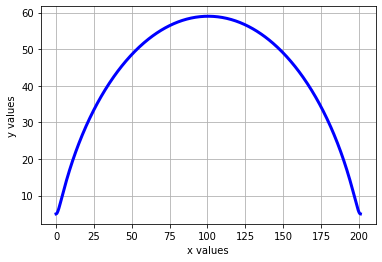
\includegraphics[width=0.5\linewidth]{Cycloid0.png}}
    \caption{Вбудовані методи креслення}
\end{figure}

\begin{figure}[h]
    \begin{minipage}[h]{0.49\linewidth}
        \center{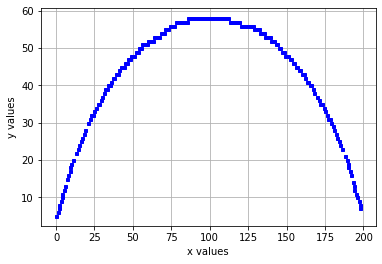
\includegraphics[width=1\linewidth]{Cycloid1.png}}
        \caption{Алгоритм Брехенхейма}
    \end{minipage}
    \hfill
    \begin{minipage}[h]{0.49\linewidth}
        \center{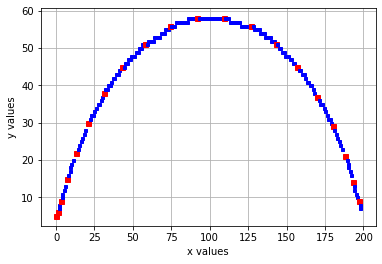
\includegraphics[width=1\linewidth]{Cycloid2.png}}
        \caption{Алгоритм Брехенхейма (мітки)}
    \end{minipage}
\end{figure}

\subsubsection*{Скріншоти кривої у полярному виді (лемініската Бернуллі)}

\begin{figure}[H]
    \center{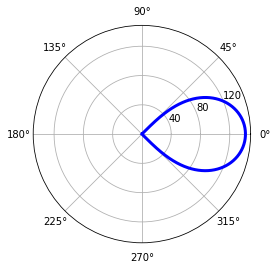
\includegraphics[width=0.5\linewidth]{Lemniscate0.png}}
    \caption{Вбудовані методи креслення}
\end{figure}

\begin{figure}[h]
    \begin{minipage}[h]{0.49\linewidth}
        \center{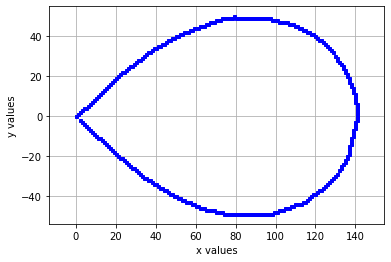
\includegraphics[width=1\linewidth]{Lemniscate1.png}}
        \caption{Алгоритм Брехенхейма}
    \end{minipage}
    \hfill
    \begin{minipage}[h]{0.49\linewidth}
        \center{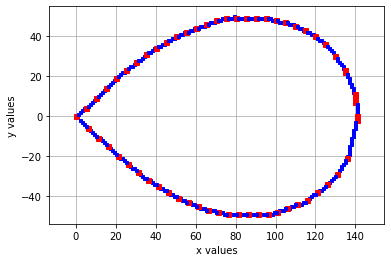
\includegraphics[width=1\linewidth]{Lemniscate2.png}}
        \caption{Алгоритм Брехенхейма (мітки)}
    \end{minipage}
\end{figure}

\subsection*{Висновки}

У лабораторному практикумі я навчився будувати криві лінії як сукупність відрізків, побудованих за 
допомогою алгоритму Брезенхема. Здобув практичні навички кодування алгоритму на мові python. Намалював 
графіки функцій, заданих рівняннями в параметричному вигляді та рівняннями у полярних координатах. Розглянув 
декілька варіантів побудови прямих в залежності від заданих початкових та кінцевих точок, розташування у 
різних квадрантах.

\subsection*{Контрольні питання}

\begin{enumerate}

    \item \textit{Для чого використовують алгоритм Брезенхейма?}

    Як і алгоритм цифрового диференціального аналізатора, алгоритм Брезенхейма теж використовують для пошуку 
    оптимальних растрових координат для представлення відрізку між двома точками.

    \item \textit{Опишіть технологію побудови відрізка прямої по алгоритму Брезенхейма.}

    Фіксуємо одну з координат, по іншій рухаємося. Задаємо певне від'ємне початкове значення помилки. Позначаємо 
    точки поточної зафіксованої прямої на кординатній сітці доти, доки значення помилки не стане додатнім. А тоді 
    корегуємо $e$ (наприклад, відніманням одиниці), і одразу збільшуємо значення зафіксованої координати.

    \item \textit{Який вид має рівняння функції у параметричному вигляді та у полярних координатах?}

    У загальному випадку рівняння функції у параметричному вигляді має вид:
    \begin{align*}   
        \begin{cases}
            x=x(t) \\ 
            y=y(t) \\
        \end{cases}, \forall t \in \mathbb{R}
    \end{align*}

    У полярних же координатах рівняння виглядає так:
    \[ \rho=\rho(\varphi),\ \varphi \in (0,2\pi),\ \rho \geqslant 0 \] 

    \item \textit{Як перетворити рівняння у полярних координатах до рівняння у параметричному вигляді та навпаки?}
    
    \begin{enumerate}
        \item полярні координати $\rightarrow$ параметричний вигляд: \par
        застосувавши для заданого рівняння $\rho(\varphi)$ нищенаведені заміни, якраз і отримаємо 
        систему у параметричному виді: 
        \begin{align*}        
            \begin{cases}
                x=\rho\cos\varphi=\rho(\varphi)\cos\varphi=x(\varphi) \\ 
                y=\rho\sin\varphi=\rho(\varphi)\sin\varphi=y(\varphi) \\
            \end{cases},\ \varphi \in (0,2\pi)
        \end{align*} 

        \item параметричний вигляд $\rightarrow$ полярні координати: \par
        із заданого у параметричному вигляді системи $x=x(\varphi),\ y=y(\varphi)$ підставляємо значення $x$ 
        та $y$ у рівняння $ \rho^2=x^2+y^2 $. Таким чином:
        \[ \rho^2=x^2+y^2=x^2(\varphi)+y^2(\varphi) \Rightarrow \rho=\rho(\varphi) \] 
    \end{enumerate}
    
    \newpage
    \item \textit{Як виконати масштабування при побудові графічних об’єктів?}
    
    Перш за все, слід віднайти поточні граничні значення вісей:
    \begin{center}
        \parbox{7cm}{\texttt{left, right = plt.xlim()\\
        down, up = plt.ylim()}}
    \end{center}
    Надалі, скажімо, за допомогою наведених нижче вбудованих функцій масштабувати графік на деякий
    коефіцієнт \texttt{alpha}:
    \begin{center}
        \parbox{9cm}{\texttt{plt.xlim(left*alpha, right*alpha)
        plt.ylim(down*alpha, up*alpha)}}
    \end{center}

\end{enumerate}

\end{document}